\subsection{Bestimmung des Planckschen Wirkungsquantums}
\subsubsection{Versuchsaufbau}
Um mithilfe des Photoeffekts das plancksche Wirkungsquantum h zu bestimmen wird der
in \cref{fig:photozelle_optikbank} skizzierte Aufbau auf einer Optikbank befestigt.
Als Lichtquelle dient eine Quecksilberdampflampe, dessen Licht nach Durchgang durch eine
Blende, mit der die Intensität des Lichts eingestellt werden kann,
mit einer Linse der Brennweite $f=\SI{100}{\milli\meter}$ auf die Kalium-Kathode
der Photozelle scharf abgebildet wird. Die Einzelnen Wellenlängen des Hg-Spektrums
werden mithilfe eines Filterrads unmittelbar vor der Photozelle selektiert,
wobei zwischen beiden Elementen ein Rohr angebracht wird, welches Streulicht
begrenzen soll. Dabei wird mit der Blende vor der Lampe sowie der Blende vor
dem Filterrad so eingestellt, dass das Licht die Kathode beleuchtet, jedoch nicht
den Anodenring oder die schwarze Fläche an der Öffnung der Schutzkappe der Photozelle.\\

Zur Spannungserzeugung steht ein \SI{12}{\volt} Netzteil zur Verfügung. Beide schwarzen
Kabel der Anode werden an den negativen Pol des Netzteils angeschlossen und
das BNC-Kabel der Kathode mit dem zur Verfügung stehenden Messverstärker.
Der andere Anschluss des Netzteils wird mit der Masse des Verstärkers angeschlossen.
Der Photostrom wird mit einem Digitalmultimeter gemessen, welches in Reihe hinter
den Verstärker geschaltet wird.
Die angeschlossene Grenzspannung wird mit einem parallel zur Spannungsquelle
geschalteten Multimeter gemessen.\\

Es ist möglich, dass ohne Photostrom des Verstärker trotzdem einen Strom ausgibt.
Mithilfe eines Tasters lässt sich die Schaltung kurzschließen, wodurch kein Strom
am Verstärker ankommt und damit an einem Regler der Ausgangsstrom in die Nulllage
kalibriert werden kann.\\

Da die vom Netzteil zu Verfügung stehenden \SI{12}{\volt} nicht vollständig in der Durchführung
ausgeschöpft werden, wird mit zwei geeigneten Widerständen ein Spannungsteiler
vorgeschaltet. Wird über dem Widerstand $R_2$ die Spannung abgegriffen, so gilt für diese
die Spannungsteilergleichung
\begin{equation}
	U = U_0\frac{R_2}{R_1 + R_2}
	\label{eq:spannungsteiler}
\end{equation}



\begin{figure}[htb]
	\centering
	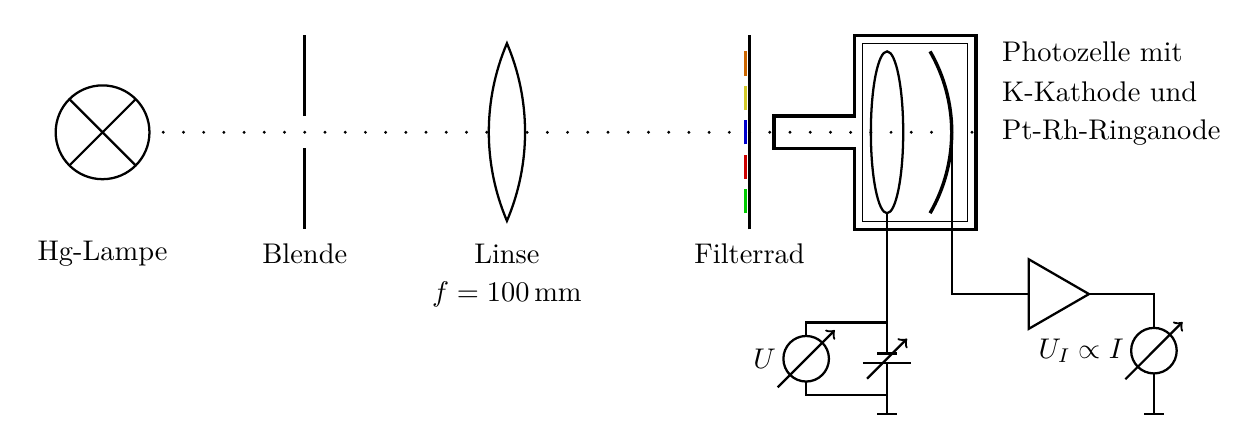
\includegraphics[width=0.8\linewidth]{../figs/photozelle_optikbank}
	\caption{Versuchsaufbau: Photoelektrische Bestimmung des planckschen Wirkungsquantum.[\textbf{QUELLE!}]}
	\label{fig:photozelle_optikbank}
\end{figure}

\subsubsection{Messung}
Im Folgenden wird mit U die am Spannungsteiler abgegriffene Spannung bezeichnet und der Photostrom 
mit I. Der Messverstärker wandelt Ströme von \SI{1}{\nano\ampere} in \SI{1}{\volt} um, 
weshalb zwar mit dem Multimeter eine Spannung gemessen wird, diese trotzdem mit einem I bezeichnet
wird. Der Strom entsteht, wenn energiereiche Photonen auf die Kathode treffen und 
Elektronen befreien, die von der Anode wieder abgefangen werden.\\ 
Beide Elektroden besitzen verschiedene Austrittsarbeiten, weshalb sich die Fermi-Niveaus
dieser unterscheiden. Bei leitender Verbindung gleichen sich die Niveaus aus, wodurch 
ein elektrisches Feld zwischen den Elektroden aufgebaut wird[\textbf{QUELLE?}]. Die Energiebilanz der eintreffenden 
Elektronen ist 
\begin{equation}
	E_\mathrm{kin} = h\nu - (W_A - W_K) - W_K = h\nu - W_A\nonumber
\end{equation}
wobei der Subskript K für die Kathode, A für die Anode und $\nu$ für die Lichtfrequenz steht.
Mit dem Netzteil wird eine Gegenspannung eingestellt und so lange erhöht, bis 
der Anodenstrom verschwindet. In diesem Falle verschwindet die kinetische Energie der Elektronen 
und es ergibt sich bei der Grenzspannung $U_0$ die Gleichung 
\begin{equation}
	eU_0 = h\nu - W_A
	\label{eq:gegenfeldmethode}
\end{equation}


\begin{figure}[htb]
	\centering
	\begin{subfigure}[c]{0.46\linewidth}
        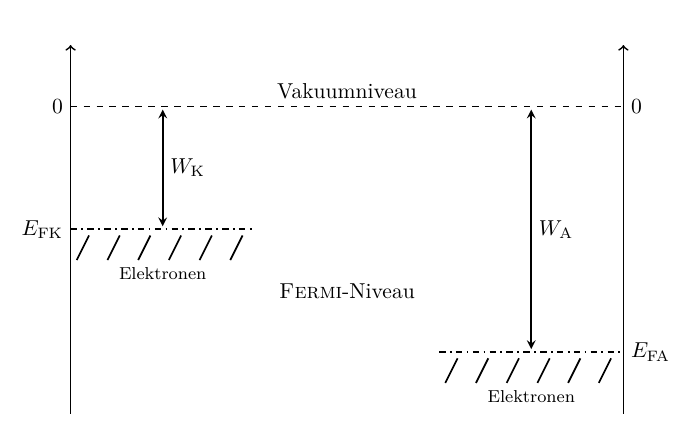
\includegraphics[width=\linewidth]{../figs/fermi1.png}
		\subcaption{nicht verbunden}
    \end{subfigure}
	\begin{subfigure}[c]{0.46\linewidth}
        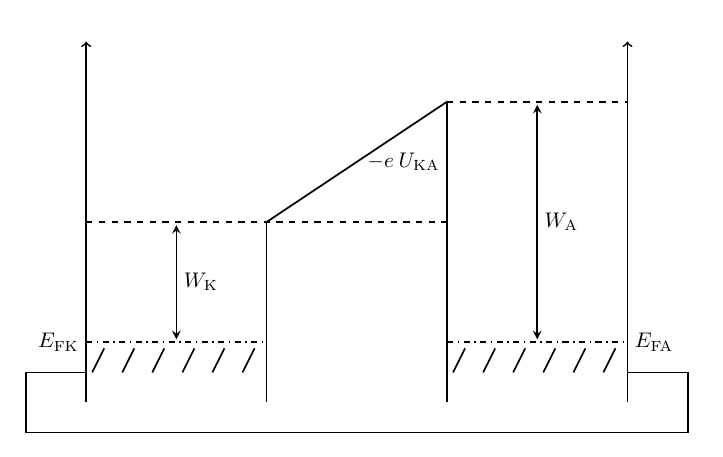
\includegraphics[width=\linewidth]{../figs/fermi2.png}
		\subcaption{leitend verbunden}
    \end{subfigure}
	\caption{Kontaktpotential zwischen zwei Elektroden}
\end{figure}

Bei dem energiereichstem Licht der Wellenlänge \SI{365}{\nano\meter} wird eine Grenzspannung von unter 
\SI{2.0}{\volt} benötigt, weshalb mit den vorhandenen Widerständen von \SI{100}{\ohm} und \SI{333}{\ohm}
nach \cref{eq:spannungsteiler} eine maximale Spannung von 
\[U_\mathrm{max} = \SI{2.77}{\volt}\]
eingestellt wird.\\
Aufgrund dessen, dass ein minimaler Anodenstrom $I_0$ auch vorhanden ist, wo Elektronen aus der 
Anode in die Kathode eintreffen, wird die Messung verfälscht. Um die Grenzspannung bestimmen zu können, 
wird für jede Wellenlänge einen Kennlinie im gesamtem Gegenspannungsbereich gemessen, angefangen 
bei \SI{0}{\volt}. Da zusätzliche Intensitätsfluktuationen auftreten können, wird jede Kennlinie 
zweimal gemessen.\\\par
Für die Wellenlänge \SI{365}{\nano\meter} wird die Messung bei einer erhöhten Intensität 
erneut gemessen, um deren Einfluss untersuchen zu können.

\subsubsection{Auswertung}

\begin{figure}[htbp]
   \centering
\caption{Kennlinie \SI{365}{nm}}
\begin{tabular}{cc||cc}
\hline\multicolumn{2}{c||}{erste Messung} & \multicolumn{2}{c}{zweite Messung}\\

\hline
$U / \unit{\milli\volt}$ & $I / \unit{\pico\ampere}$ & $U / \unit{\milli\volt}$ & $I / \unit{\pico\ampere}$ \\ 
\hline
$\num{0}$ & $\num{732\pm 3}$ & $\num{0}$ & $\num{732\pm 4}$ \\
$\num{107}$ & $\num{638\pm 4}$ & $\num{120}$ & $\num{613\pm 4}$ \\
$\num{203}$ & $\num{556\pm 2}$ & $\num{242}$ & $\num{510\pm 3}$ \\
$\num{343}$ & $\num{436\pm 5}$ & $\num{381}$ & $\num{402\pm 2}$ \\
$\num{439}$ & $\num{375\pm 5}$ & $\num{497}$ & $\num{321\pm 1}$ \\
$\num{572}$ & $\num{282\pm 2}$ & $\num{615}$ & $\num{250\pm 1}$ \\
$\num{721}$ & $\num{198\pm 2}$ & $\num{733}$ & $\num{186\pm 1}$ \\
$\num{853}$ & $\num{135\pm 5}$ & $\num{861}$ & $\num{127\pm 1}$ \\
$\num{1003}$ & $\num{82\pm 5}$ & $\num{1057}$ & $\num{62.5\pm 0.5}$ \\
$\num{1210}$ & $\num{33\pm 4}$ & $\num{1299}$ & $\num{22.5\pm 0.5}$ \\
$\num{1322}$ & $\num{15\pm 2}$ & $\num{1340}$ & $\num{10.5\pm 0.5}$ \\
$\num{1440}$ & $\num{1.1\pm 0.5}$ & $\num{1430}$ & $\num{-1.2\pm 0.4}$ \\
$\num{1589}$ & $\num{-17.4\pm 0.3}$ & $\num{1498}$ & $\num{-10.2\pm 0.5}$ \\
$\num{1761}$ & $\num{-20.6\pm 0.4}$ & $\num{1624}$ & $\num{-20.0\pm 0.5}$ \\
$\num{2016}$ & $\num{-20.9\pm 0.3}$ & $\num{1542}$ & $\num{-14.9\pm 0.3}$ \\
$\num{2782}$ & $\num{-21.2\pm 0.4}$ & $\num{1914}$ & $\num{-21.5\pm 0.2}$ \\
   &    & $\num{2783}$ & $\num{-21.9\pm 0.2}$ \\
\hline\end{tabular}
\label{kennlinie_365nm}
\end{figure}
\doublefigure{365_1}{365_2}{365}

Aus den Kennlinien der Photozelle lässt sich die Grenzspannung bestimmen. In \cref{kennlinie_365nm} sind die 
Messreihen bei einem Filter bei \SI{365}{\nano\meter} dargestellt (die restlichen Messdaten sind im Anhang 
\ref{sec:anhang_photozelle} zu finden). Die Spannungsmessung besitzt lediglich einen Ablesefehler der letzten 
angezeigten Ziffer, weshalb der Fehler jedes Messwertes bei $\Delta U = \SI{1}{\milli\volt}$ liegt.
Die Strommessung war teilweise starken Fluktuationen ausgesetzt, weshalb der Fehler $\Delta I$
individuell an diese Schwankung angepasst wird. Für die meisten Messwerte bestimmt somit der Fehler 
des Photostroms die größte Unsicherheit, da der zur Messgröße relative Fehler deutlich größer ausfällt.\\
Im Anlaufgebiet der Photozelle wächst der Strom quadratisch mit der Gegenspannung an[\textbf{QUELLE}],
weshalb für die Wurzel dessen ein linearer Zusammenhang der Form 
\begin{equation}
	\sqrt{I - I_0} = m\cdot U + b \nonumber
\end{equation}
erwartet wird, wobei $I_0$ bei maximaler eingesteller Gegenspannung abgelesen wird.
Nach Gaußscher Fehlerfortpflanzung[\textbf{QUELLE}] gilt für den dazugehörigen Fehler
\begin{equation}
	\Delta\sqrt{I - I_0} = \sqrt{\qty(\frac{\Delta I}{\sqrt{I-I_0}})^2 + \qty(\frac{\Delta I_0}{\sqrt{I-I_0}})^2} \nonumber
\end{equation}

Für die erste Wellenlänge sind die Kennlinien in \cref{fig:kennlinie_365} mit einer Ausgleichsgeraden 
dargestellt, wobei zur Bestimmung der Geraden nur Werte in dem linearen Bereich in Betracht gezogen wurden
(Weitere Kennlinien befinden sich im Anhang \ref{sec:anhang_photozelle} 
\crefrange{fig:kennlinie_405}{fig:kennlinie_578}). Aus der Nullstelle der Geraden wird die Grenzspannung 
bestimmt mit 
\begin{equation}
	U_0 = - \frac{b}{m},\qquad \Delta U_0 = \sqrt{\qty(\frac{\Delta b}{m})^2 + \qty(\frac{b\Delta m}{m^2})^2}
	\label{eq:bestimmung_grenzspannung}
\end{equation}
